\FloatBarrier
\begin{figure}[!h]
\centering
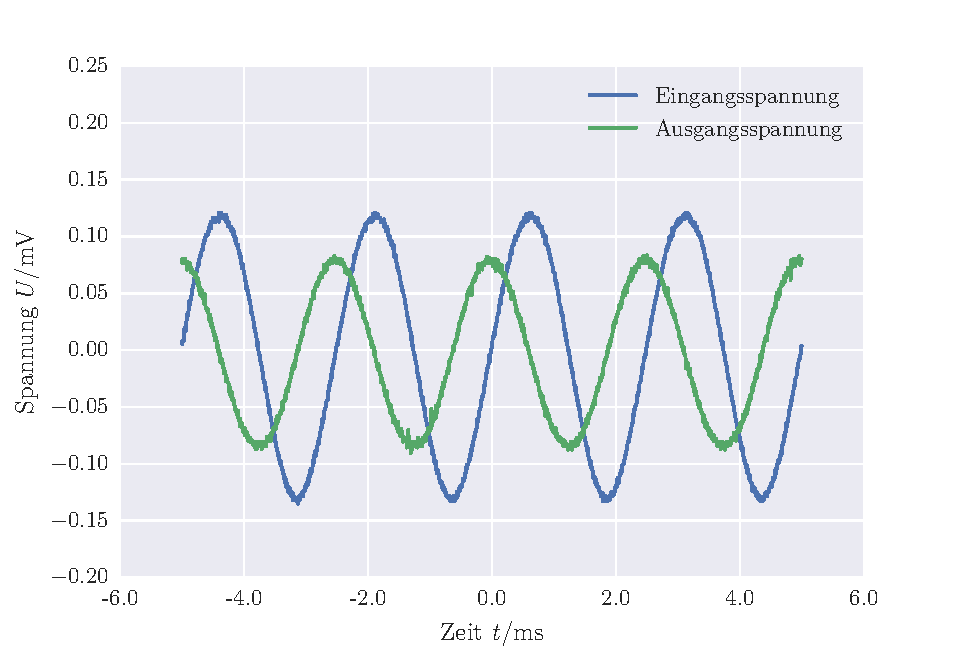
\includegraphics[scale=0.75]{../Grafiken/Integrator_Oszilloskop_Sinus.pdf}
\caption{Vom Oszilloskop aufgenommene Ein- und Ausgangsspannungen der Integratorschaltung. Auf dem Eingang
	liegt hier eine Sinusspannung. Die Ausgangsspannung in Form eines Kosinus entspricht dem theoretisch
	zu erwartendem Verlauf.
	 \label{fig:integrator_oszilloskop_sinus}}
\end{figure}
\FloatBarrier